% Source: :contentReference[oaicite:0]{index=0}
\documentclass{article}
\usepackage{amsmath,amssymb,graphicx,tikz,pgfplots,booktabs,xcolor}
\pgfplotsset{compat=1.18}

\newenvironment{lesson-meta}{}{}        % lesson code, title, objective, EQ, vocab
\newenvironment{item-analysis}{}{}      % Savvas's Example × DOK table
\newenvironment{model-discuss}{}{}      % Launch opener
\newenvironment{concept-box}{}{}        % in-lesson concept reference
\newenvironment{concept-summary}{}{}    % end-of-lesson summary
\newenvironment{example}[1]{}{}         % #1 = example number
\newenvironment{tryit}[1]{}{}           % #1 = tryit number
\newenvironment{practice}[2]{}{}        % #1 = practice number, #2 = DOK
\newenvironment{te-addendum}[2]{}{}     % #1 = anchor example, #2 = type
\newcommand{\answer}[1]{}               % answer key, inside any env
\newcommand{\placeholder}[2]{}          % #1 = type, #2 = description
\newcommand{\uncertain}[2]{#1}          % #1 = best guess, #2 = alternatives
\newcommand{\te}[1]{}                   % teacher-only inline annotation

\begin{document}

\begin{lesson-meta}
Lesson Code: 6-5

Title: Properties of Logarithms

I CAN: use properties of logarithms to rewrite expressions.

Objective: Use Properties of Logarithms to rewrite logarithmic expressions. Use the Change of Base Formula to evaluate logarithmic expressions and solve equations.

Essential Question: How are properties of logarithms used to simplify expressions and solve logarithmic equations?

Lesson Vocabulary: Change of Base Formula

Topic Vocabulary: logarithm; power; product; quotient
\end{lesson-meta}

\begin{item-analysis}
\begin{tabular}{ccc}
\toprule
Example & Items & DOK \\
\midrule
1 & 13 & 3 \\
2 & 14--17 & 1 \\
2 & 7, 9 & 2 \\
3 & 18--22, 39 & 1 \\
3 & 8, 11, 37 & 2 \\
4 & 23, 36, 40 & 2 \\
5 & 24--29, 38 & 1 \\
5 & 12 & 2 \\
6 & 30--35 & 1 \\
6 & 10 & 2 \\
\bottomrule
\end{tabular}
\end{item-analysis}

\begin{model-discuss}
EXPLORE AND REASON

Look at the graph of $y=\log x$ and the ordered pairs shown.

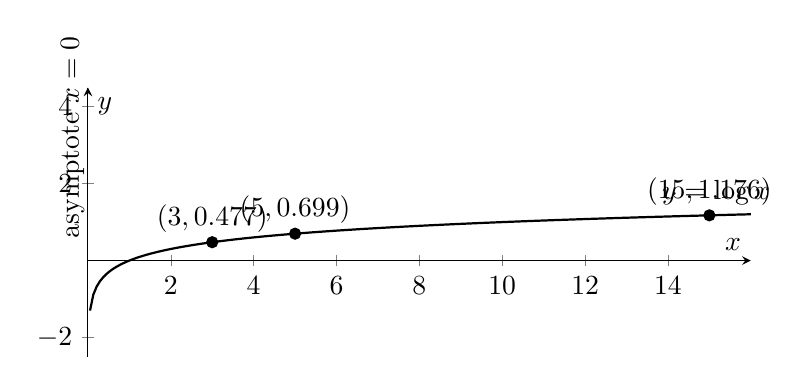
\begin{tikzpicture}
\begin{axis}[
    axis lines=middle,
    xmin=0, xmax=16,
    ymin=-2.5, ymax=4.5,
    xlabel={$x$}, ylabel={$y$},
    xtick={0,2,4,6,8,10,12,14},
    ytick={-2,0,2,4},
    domain=0.05:16,
    samples=200,
    width=10cm,
    height=5cm,
    clip=false
]
\addplot[thick] {log10(x)} node[pos=0.95, above] {$y=\log x$};
\addplot[only marks, mark=*] coordinates {(3,0.477) (5,0.699) (15,1.176)};
\node[above] at (axis cs:3,0.477) {$(3,0.477)$};
\node[above] at (axis cs:5,0.699) {$(5,0.699)$};
\node[above] at (axis cs:15,1.176) {$(15,1.176)$};
\addplot[dashed] coordinates {(0,-2.5) (0,4.5)};
\node[rotate=90, anchor=south] at (axis cs:0.15,3.2) {asymptote $x=0$};
\end{axis}
\end{tikzpicture}

A. Complete the table shown.

\begin{tabular}{c|ccc}
$x$ & 3 & 5 & 15 \\
\hline
$\log x$ & & & \\
\end{tabular}

B. Look for Relationships What is the relationship between the numbers 3, 5, and 15? What is the relationship between the logarithms of 3, 5, and 15?

C. What is your prediction for the value of $\log 45$? $\log 75$? Explain.

\answer{A. \(\begin{array}{c|ccc}x&3&5&15\\\hline \log x&0.477&0.699&1.176\end{array}\) B. \(3\times5=15\), so 3 and 5 are both factors of 15. \(0.477+0.699=1.176\), so \(\log3+\log5=\log15\). C. I know that \(45=3\times15\), so \(\log45\) is the same as \(\log3+\log15\), meaning the value of \(\log45\) is 1.653. And \(75=5\times15\), so \(\log75=\log5+\log15\), or about 1.875.}
\end{model-discuss}

\begin{te-addendum}{ModelDiscuss}{PurposefulQuestions}
Q: What are some of the features of the graph of $y=\log x$?
\answer{The graph has an $x$-intercept at 1 and vertical asymptote at the $y$-axis.}
Q: What kinds of problems is a graph or a table useful in solving?
\answer{Sample: problems that require you to find a pattern.}
\end{te-addendum}

\begin{te-addendum}{ModelDiscuss}{PurposefulQuestions}
Q: What do you notice about the labeled points on the graph?
\answer{The $x$-values 3 and 5 are factors of 15.}
\end{te-addendum}

\begin{te-addendum}{ModelDiscuss}{RtIExtend}
Q: Choose four composite numbers. Find the logarithm of the numbers and the logarithms of a pair of their factors. Make a table of your results. Are your results the same as in Part B?
\answer{Yes; the sum of logarithms of the factors is equal to the logarithm of the number.}
\end{te-addendum}

\begin{te-addendum}{ModelDiscuss}{PurposefulQuestions}
Q: What do you notice about the values of $\log x$ in the table?
\answer{The sum of the first two values of $\log x$ is equal to the third value of $\log x$.}
Q: How did you apply what you discovered in Part B to Part C?
\answer{Sample: In Part B, I determined that the sum of the logs of two factors is equal to the log of their product. Because 3 and 15 are factors of 45, I predicted $\log45$ would equal $\log3+\log15$. Similarly, I predicted $\log75$ would equal $\log5+\log15$.}
\end{te-addendum}

\begin{te-addendum}{ModelDiscuss}{HabitsOfMind}
Generalize Do you think that the relationships you found in the Explore \& Reason activity would also hold for natural logarithms? Give an example.
\answer{yes; $\ln3+\ln5=\ln15$}
\end{te-addendum}

\begin{concept-box}
CONCEPT Properties of Logarithms

For positive numbers $b$, $m$, and $n$ with $b\neq1$, the following properties hold.

\begin{tabular}{ll}
Product Property of Logarithms & $\log_b(mn)=\log_b m+\log_b n$ \\
Quotient Property of Logarithms & $\log_b\left(\dfrac{m}{n}\right)=\log_b m-\log_b n$ \\
Power Property of Logarithms & $\log_b(m^n)=n\log_b m$ \\
\end{tabular}
\end{concept-box}

\begin{te-addendum}{EssentialQuestion}{PurposefulQuestions}
Q: What do you notice about the Product Property of Logarithms?
\answer{The log of a product equals the sum of the logs of the factors.}
\end{te-addendum}

\begin{example}{1}
Prove a Property of Logarithms

How can you prove the Product Property of Logarithms?

Let $x=\log_b m$ and $y=\log_b n$. Then $b^x=m$ and $b^y=n$.

\[
\begin{aligned}
b^x\cdot b^y&=m\cdot n && \text{Multiply the expressions } b^x \text{ and } b^y.\\
b^{x+y}&=mn\\
x+y&=\log_b mn && \text{Rewrite the equation in logarithmic form.}\\
\log_b m+\log_b n&=\log_b mn
\end{aligned}
\]

\answer{$\log_b m+\log_b n=\log_b mn$}
\end{example}

\begin{te-addendum}{1}{ElicitEvidence}
Q: Why would the equations $x=\log_b m$ and $y=\log_b n$ be used to start the proof?
\answer{These expressions can be rewritten as exponential equations with a common base. The Product Property of Exponents can then be used to complete the proof.}
\end{te-addendum}

\begin{te-addendum}{1}{LearnTogether}
Listen Actively When you listen actively, you try to understand what the other person means. Ask What can you do to make sure you hear and understand someone's idea? What can you do or say if you still don't understand?
\end{te-addendum}

\begin{tryit}{1}
Prove the Quotient Property of Logarithms.

\answer{Let \(x=\log_b m\) and \(y=\log_b n\). Then \(b^x=m\) and \(b^y=n\). \(\begin{aligned}\frac{b^x}{b^y}&=\frac{m}{n}\\ b^{x-y}&=\frac{m}{n}\\ x-y&=\log_b\left(\frac{m}{n}\right)\\ \log_b m-\log_b n&=\log_b\left(\frac{m}{n}\right)\end{aligned}\)}
\end{tryit}

\begin{te-addendum}{2}{PurposefulQuestions}
Additional Example 2 Use properties of logarithms to expand the expression $\log_5\left(\dfrac{9x^8}{y^9}\right)$.
\answer{$\log_5\left(\dfrac{9x^8}{y^9}\right)=\log_5 9+\log_5 x^8-\log_5 y^9=\log_5 3^2+\log_5 x^8-\log_5 y^9=2\log_5 3+8\log_5 x-9\log_5 y$}
Q: Which property should you apply first?
\answer{Apply the Quotient Property of Logarithms first to remove the fraction.}
\end{te-addendum}

\begin{example}{2}
Expand Logarithmic Expressions

How can you use the properties of logarithms to expand each expression?

A. $\log_5(a^2b^7)$
\[
\begin{aligned}
\log_5(a^2b^7)&=\log_5(a^2)+\log_5(b^7)\\
&=2\log_5 a+7\log_5 b
\end{aligned}
\]

B. $\ln\left(\dfrac{25}{3}\right)$
\[
\begin{aligned}
\ln\left(\frac{25}{3}\right)&=\ln\left(\frac{5^2}{3}\right)\\
&=\ln(5^2)-\ln3\\
&=2\ln5-\ln3
\end{aligned}
\]

\answer{A. $2\log_5 a+7\log_5 b$; B. $2\ln5-\ln3$}
\end{example}

\begin{te-addendum}{2}{PurposefulQuestions}
Q: Why might it be useful to know how to expand logarithmic expressions?
\answer{It may be easier to solve logarithmic equations when each side is written in expanded form.}
\end{te-addendum}

\begin{tryit}{2}
Use the properties of logarithms to expand each expression.

A. $\log_7\left(\dfrac{r^3t^4}{v}\right)$

B. $\ln\left(\dfrac{7}{225}\right)$

\answer{A. $3\log_7 r+4\log_7 t-\log_7 v$; B. $\ln7-2\ln3-2\ln5$}
\end{tryit}

\begin{example}{3}
Write Expressions as Single Logarithms

What is each expression written as a single logarithm?

A. $4\log_4 m+3\log_4 n-\log_4 p$
\[
\begin{aligned}
4\log_4 m+3\log_4 n-\log_4 p
&=\log_4(m^4)+\log_4(n^3)-\log_4 p\\
&=\log_4(m^4n^3)-\log_4 p\\
&=\log_4\left(\frac{m^4n^3}{p}\right)
\end{aligned}
\]

B. $3\ln2-2\ln5$
\[
\begin{aligned}
3\ln2-2\ln5&=\ln(2^3)-\ln(5^2)\\
&=\ln\left(\frac{2^3}{5^2}\right)\\
&=\ln\left(\frac{8}{25}\right)
\end{aligned}
\]

\answer{A. $\log_4\left(\dfrac{m^4n^3}{p}\right)$; B. $\ln\left(\dfrac{8}{25}\right)$}
\end{example}

\begin{te-addendum}{3}{PurposefulQuestions}
Q: How do the processes of expanding a logarithm and writing an expression as a single logarithm relate to each other?
\answer{The process of writing expressions as single logarithms is the reverse of the process of expanding logarithmic expressions.}
\end{te-addendum}

\begin{te-addendum}{3}{ElicitEvidence}
Q: Is it necessary to apply the Property of Logarithms in a specific order?
\answer{Sample: Yes, you cannot apply the Quotient Property until after you apply the Power Property.}
\end{te-addendum}

\begin{te-addendum}{3}{HabitsOfMind}
Make Sense and Persevere Using the fact that $\log2\approx0.3010$ and $\log3\approx0.4771$, what is $\log18$? Explain.
\answer{approx. 1.2553; since $18=2\times3\times3$, $\log18=\log2+\log3+\log3$}
\end{te-addendum}

\begin{te-addendum}{3}{ELLAddendum}
SPEAKING BEGINNING In small groups, ask students to discuss how many different meanings of the word log they can think of. Encourage them to think of how log can be used as a noun and how it can be used as a verb.
Q: What are some meanings for the word log your group came up with?
\answer{part of a tree trunk, a recording of data or events, a device that determines the speed of a ship, to cut trees down, to keep a record of, to make a certain speed or travel for a certain amount of time}
Q: Why do we call a logarithm a log when we mean something completely different?
\answer{Log is like a nickname for logarithm.}

LISTENING DEVELOPING Review the example and the study tip. Draw students' attention to the words single and signal. Provide sentence frames for students to complete with either single or signal (i.e. A red light \underline{\hspace{1cm}} a car to stop. He was so quiet he didn't say a \underline{\hspace{1cm}} word.).
Q: Do signals give information?
\answer{Yes; they tell us when to stop and to go.}
Q: Is the word multiple similar to the word single?
\answer{No; they are antonyms.}

WRITING EXPANDING After reviewing the example and the study tip, have students spend 2 to 5 minutes writing about how they could use the signals in the problem to write single logarithms.
Q: Why are the expressions at the beginning of the examples not considered to be single?
\answer{They are expressions with more than one term.}
Q: What signals should you look for first when simplifying an expression to a single logarithm?
\answer{multiplication by a constant to signal the Power Property}
\end{te-addendum}

\begin{tryit}{3}
Write each expression as a single logarithm.

A. $5\log_2 c-7\log_2 n$

B. $2\ln7+\ln2$

\answer{A. $\log_2\left(\dfrac{c^5}{n^7}\right)$; B. $\ln98$}
\end{tryit}

\begin{te-addendum}{3}{RtIExtend}
USE WITH EXAMPLE 3 Have students explore the effect of parentheses on writing expressions as single logarithms.

Give students these examples.

$4\log x+3\log2-(2\log y+\log5)$

Q: Write this expression as a single logarithm.
\answer{$\log\left(\dfrac{8x^4}{5y^2}\right)$}
Q: Write $4\log x+3\log2-2\log y+\log5$ as a single expression.
\answer{$\log\left(\dfrac{40x^4}{y^2}\right)$}
Q: How did removing the parentheses from $4\log x+3\log2-(2\log y+\log5)$ affect writing the expression as a single logarithm?
\answer{Removing the parentheses changed the expression to have only one factor in the denominator.}
\end{te-addendum}

\begin{example}{4}
Apply Properties of Logarithms

PH OF A SOLUTION The pH of a solution is a measure of its concentration of hydrogen ions. This concentration (measured in moles per liter) is written $[H^+]$ and is given by the formula
\[
\mathrm{pH}=\log\frac{1}{[H^+]}.
\]
What is the concentration of hydrogen ions in the acid rainfall?

\placeholder{illustration}{pH of a solution graphic showing orange juice pH = 3, acid rain pH = 4.5, clear rain pH = 5.6, and healthy lake pH = 6.5.}

Solve for $[H^+]$.
\[
\begin{aligned}
4.5&=\log\frac{1}{[H^+]}\\
4.5&=\log1-\log[H^+]\\
-4.5&=\log[H^+]\\
10^{-4.5}&=[H^+]
\end{aligned}
\]
The concentration of hydrogen ions in the acid rainfall is $10^{-4.5}\approx0.0000316$ moles per liter.

\answer{$10^{-4.5}\approx0.0000316$ moles per liter}
\end{example}

\begin{te-addendum}{4}{PurposefulQuestions}
Q: What does the $+$ in $H^+$ represent? Does it affect how you solve the equation?
\answer{$H^+$ is the concentration of hydrogen ions in a solution. The $+$ indicates that the hydrogen ions have a positive charge. $H^+$ is a variable, so the $+$ does not affect how the equation is solved.}
\end{te-addendum}

\begin{te-addendum}{4}{CommonError}
The expression $\log\dfrac{1}{[H^+]}$ is equal to $\log1-\log[H^+]$, not $\log[1-H^+]$.
\end{te-addendum}

\begin{te-addendum}{4}{HabitsOfMind}
Generalize What types of numbers have logarithms that are negative? Explain.
\answer{Real numbers between 0 and 1; a positive number raised to a negative exponent is equal to a number between 0 and 1.}
\end{te-addendum}

\begin{tryit}{4}
What is the concentration of hydrogen ions in a liter of orange juice?

\answer{$10^{-3}$ moles per liter, or 0.001 moles per liter}
\end{tryit}

\begin{concept-box}
Evaluate Logarithmic Expressions by Changing the Base

How can you use base 10 logarithms to evaluate base 2 logarithms?

To evaluate $\log_2 3$ with a calculator, you need to express $\log_2 3$ in terms of base 10 logarithms.
\end{concept-box}

\begin{example}{5}
Evaluate Logarithmic Expressions by Changing the Base

\[
\begin{aligned}
\log_2 3
&=\frac{\log_2 3\cdot\log2}{\log2}\\
&=\frac{\log 2^{\log_2 3}}{\log2}\\
&=\frac{\log3}{\log2}\\
&=\frac{0.477}{0.301}\approx1.585
\end{aligned}
\]

Remember that exponents and logarithms are inverse operations, so they undo one another.

This illustrates the Change of Base Formula:

For positive numbers $m$, $b$, and $a$, with $b\neq1$ and $a\neq1$,
\[
\log_b m=\frac{\log_a m}{\log_a b}.
\]

\answer{$\log_2 3\approx1.585$}
\end{example}

\begin{te-addendum}{5}{PurposefulQuestions}
Q: What does each variable represent when you use the Power Property of Logarithms?
\answer{$n=\log_2 3$, $b=10$, and $m=2$}
\end{te-addendum}

\begin{te-addendum}{5}{ElicitEvidence}
Q: Do you need to go through all of the steps shown in the example to complete the Try It? Explain.
\answer{No; The example illustrated how the Change of Base Formula was derived. To complete the Try It, the formula can be used directly.}
\end{te-addendum}

\begin{te-addendum}{5}{RtISupport}
USE WITH EXAMPLE 5 Some students have difficulty understanding the Change of Base Formula.

Have students analyze each step of the process of deriving the Change of Base Formula.

Q: What is the purpose of multiplying by 1 in the form of $\dfrac{\log2}{\log2}$?
\answer{Most calculators cannot evaluate logs with a base of 2, so multiplying by $\dfrac{\log2}{\log2}$ is the first step in rewriting the expression with a base of 10.}
Q: Explain how to move from the second step to the third step.
\answer{Exponents and logarithms are inverse operations, so in the expression $\log 2^{\log_2 3}$, the exponent of $\log_2$ undoes the 2, leaving only $\log3$.}
Q: Why can you use a calculator to evaluate $\dfrac{\log3}{\log2}$?
\answer{Both logarithms have a base of 10, which a calculator can evaluate.}
\end{te-addendum}

\begin{tryit}{5}
Estimate the value of each logarithm. Then use a calculator to find the value of each logarithm to the nearest thousandth.

A. $\log_2 7$

B. $\log_5 3$

\answer{A. 2.807; B. 0.683}
\end{tryit}

\begin{te-addendum}{6}{PurposefulQuestions}
Additional Example 6 Solve $3^x=10$ using common logarithms. Then solve $3^x=10$ using natural logarithms. Explain the results.
\answer{$x=\log_3 10=\dfrac{\log10}{\log3}\approx2.096$ and $x=\log_3 10=\dfrac{\ln10}{\ln3}\approx2.096$. You can solve an exponential equation by using common logarithms or by using natural logarithms because both methods give the same answer.}
Q: What would the solution be if you used base 2?
\answer{The solution would be the same.}
\end{te-addendum}

\begin{example}{6}
Use the Change of Base Formula

What is the solution of the equation $2^x=7$? Express the solution as a logarithm and then evaluate. Round to the nearest thousandth.

\[
\begin{aligned}
2^x&=7\\
x&=\log_2 7\\
x&=\frac{\log7}{\log2}\\
x&\approx2.807
\end{aligned}
\]

Check: $2^{2.807}\approx7$.

\answer{$x=\log_2 7=\dfrac{\log7}{\log2}\approx2.807$}
\end{example}

\begin{te-addendum}{6}{PurposefulQuestions}
Q: Why can you solve the equation using both base 10 logarithms and natural logarithms?
\answer{According to the Change of Base Formula, the only restrictions on the base are that it is positive and it cannot equal 1. So logarithms of base 10, $e$, or any other base can be used.}
\end{te-addendum}

\begin{te-addendum}{6}{CommonError}
Try It! 6 Students may divide each side by the base of the exponent instead of using logarithms. Emphasize that the equation is an exponential equation and that logarithms are the inverse of exponents.
\end{te-addendum}

\begin{te-addendum}{6}{HabitsOfMind}
Use Appropriate Tools Why is the Change of Base Formula useful when evaluating a logarithm with a calculator?
\answer{Standard calculators do not have an option to take the logarithm of something with a base other than 10 or $e$, so the Change of Base Formula gives you a way to solve the expression using a calculator.}
\end{te-addendum}

\begin{tryit}{6}
What is the solution to the equation $3^x=15$? Express the solution as a logarithm, make an estimate, and then evaluate. Round to the nearest thousandth.

\answer{$\dfrac{\log15}{\log3}$; 2.465}
\end{tryit}

\begin{concept-summary}
CONCEPT SUMMARY Properties of Logarithms

\begin{tabular}{p{0.18\linewidth}p{0.19\linewidth}p{0.19\linewidth}p{0.19\linewidth}p{0.19\linewidth}}
\toprule
& Product Property & Quotient Property & Power Property & Change of Base \\
\midrule
ALGEBRA & $\log_b(mn)=\log_b m+\log_b n$ & $\log_b\left(\dfrac{m}{n}\right)=\log_b m-\log_b n$ & $\log_b(m^n)=n\cdot\log_b m$ & $\log_b m=\dfrac{\log_a m}{\log_a b}$ \\
WORDS & The log of a product is the sum of the logs. & The log of a quotient is the difference of the logs. & The log of a number raised to a power is the power multiplied by the log of the number. & The log base $b$ of a number is equal to the log base $a$ of the number divided by the log base $a$ of $b$. \\
NUMBERS & $\log_2(20)=\log_2(4)+\log_2(5)$ & $\log_{10}\left(\dfrac{2}{3}\right)=\log_{10}2-\log_{10}3$ & $\log_3(16)=4\cdot\log_3 2$ & $\log_5 7=\dfrac{\log7}{\log5}$ \\
\bottomrule
\end{tabular}
\end{concept-summary}

\begin{te-addendum}{ConceptSummary}{PurposefulQuestions}
Q: How are the properties of logarithms useful when solving problems?
\answer{The properties of logarithms help you rewrite logarithms into forms that are more useful to solve specific problems. The Change of Base formula can be used to estimate the value of a logarithm.}
\end{te-addendum}

\begin{te-addendum}{DoYouKnowHow5}{CommonError}
Exercise 5 Students may incorrectly use the product property to write the expression as $\ln(30st)$ instead of $\ln(s^5t^6)$. Explain that the first step is to rewrite $5\ln s+6\ln t$ as $\ln s^5+\ln t^6$ using the product property.
\end{te-addendum}

\begin{practice}{7}{2}
Use Structure Without applying the Change of Base Formula, explain how to use $\log_3 2\approx0.631$ and $\log_3 5\approx1.465$ to approximate $\log_3\left(\dfrac{2}{5}\right)$.

\answer{Use the Quotient Property to rewrite $\log_3\left(\dfrac{2}{5}\right)$ as $\log_3 2-\log_3 5$. Substitute 0.631 for $\log_3 2$ and 1.465 for $\log_3 5$, then subtract to approximate the logarithm as $-0.834$.}
\end{practice}

\begin{practice}{8}{2}
Communicate Precisely Explain what is meant by expanding a logarithmic expression. How are the processes of expanding logarithmic expressions and writing logarithmic expressions as a single logarithm related?

\answer{To expand, separate the factors inside the logarithm into separate sums of logarithms. To write a single logarithmic expression, combine sums of logarithms into a single logarithm of the product.}
\end{practice}

\begin{practice}{9}{2}
Higher Order Thinking The graph of $y=\log\left(\dfrac{1}{x}\right)$ and $y=-\log x$ are shown. Notice the graph is the same for both equations. Use properties of logarithms to explain why the graphs are the same.

\begin{tikzpicture}
\begin{axis}[
    axis lines=middle,
    xmin=-4.5, xmax=4.5,
    ymin=-4.5, ymax=4.5,
    xlabel={$x$}, ylabel={$y$},
    xtick={-4,-2,0,2,4},
    ytick={-4,-2,0,2,4},
    domain=0.08:4.5,
    samples=200,
    width=7cm,
    height=6cm,
    clip=false
]
\addplot[thick] {-log10(x)} node[pos=0.9, below] {$y=\log\left(\frac{1}{x}\right)=-\log x$};
\addplot[dashed] coordinates {(0,-4.5) (0,4.5)};
\node[rotate=90, anchor=south] at (axis cs:0.15,3.4) {asymptote $x=0$};
\end{axis}
\end{tikzpicture}

\answer{$y=\log\left(\dfrac{1}{x}\right)=\log1-\log x=0-\log x=-\log x$}
\end{practice}

\begin{practice}{10}{2}
Communicate Precisely Saachi used the Change of Base Formula to solve the equation $6^x=72$ and found that $x=2.387$. How can Saachi check her solution?

\answer{Saachi can check if $6^{2.387}=72$.}
\end{practice}

\begin{practice}{11}{2}
Error Analysis Describe and correct the error a student made in writing the logarithmic expression in terms of a single logarithm.

\[
\log_3 2+\frac{1}{2}\log_3 y=\log_3 2y^2
\]

\answer{The student used 2 as an exponent instead of $\frac{1}{2}$. The correct expression is $\log_3(2y^{1/2})$.}
\end{practice}

\begin{practice}{12}{2}
Error Analysis A student wants to approximate $\log_2 9$ with her calculator. She enters the equivalent expression $\dfrac{\ln2}{\ln9}$, but the decimal value is not close to her estimate of 3. What happened?

\[
\log_2 9=\frac{\ln2}{\ln9}
\]

\answer{The student applied the change of base property incorrectly.}
\end{practice}

\begin{practice}{13}{3}
Use the properties of exponents to prove the Power Property of Logarithms.

\answer{Let \(\log_b(m^n)=x\). \(\begin{aligned} b^x&=m^n\\ (b^x)^{1/n}&=(m^n)^{1/n}\\ b^{x/n}&=m\\ \frac{x}{n}&=\log_b m\\ x&=n\log_b m\\ \log_b(m^n)&=n\log_b(m)\end{aligned}\)}
\end{practice}

\begin{practice}{14}{1}
Use the properties of logarithms to expand each expression.

$\log_5\left(\dfrac{2}{3}\right)$

\answer{$\log_5 2-\log_5 3$}
\end{practice}

\begin{practice}{15}{1}
Use the properties of logarithms to expand each expression.

$\log_6(2m^5n^3)$

\answer{$\log_6 2+5\log_6 m+3\log_6 n$}
\end{practice}

\begin{practice}{16}{1}
Use the properties of logarithms to expand each expression.

$\ln 2x^5$

\answer{$\ln2+5\ln x$}
\end{practice}

\begin{practice}{17}{1}
Use the properties of logarithms to expand each expression.

$\log_2\left(\dfrac{x}{5y}\right)$

\answer{$\log_2 x-\log_2 5-\log_2 y$}
\end{practice}

\begin{practice}{18}{1}
Use the properties of logarithms to write each expression as a single logarithm.

$9\ln x-6\ln y$

\answer{$\ln\left(\dfrac{x^9}{y^6}\right)$}
\end{practice}

\begin{practice}{19}{1}
Use the properties of logarithms to write each expression as a single logarithm.

$\log_5 6+\dfrac{1}{2}\log_5 y$

\answer{$\log_5(6y^{1/2})$}
\end{practice}

\begin{practice}{20}{1}
Use the properties of logarithms to write each expression as a single logarithm.

$2\log10+4\log(3x)$

\answer{$\log(8100x^4)$}
\end{practice}

\begin{practice}{21}{1}
Use the properties of logarithms to write each expression as a single logarithm.

$\dfrac{1}{3}\ln27-3\ln(2y)$

\answer{$\ln\left(\dfrac{3}{8y^3}\right)$}
\end{practice}

\begin{practice}{22}{1}
Use the properties of logarithms to write each expression as a single logarithm.

$8\log_3 2+5\log_3 c+7\log_3 d$

\answer{$\log_3(256c^5d^7)$}
\end{practice}

\begin{practice}{23}{2}
Use properties of logarithms to show that $\mathrm{pH}=\log\dfrac{1}{[H^+]}$ can be written as $\mathrm{pH}=-\log[H^+]$.

\answer{$\mathrm{pH}=\log\left(\dfrac{1}{[H^+]}\right)=\log1-\log[H^+]=0-\log[H^+]=-\log[H^+]$}
\end{practice}

\begin{practice}{24}{1}
Use the Change of Base Formula to evaluate each logarithm. Round to the nearest thousandth.

$\log_4 9$

\answer{1.585}
\end{practice}

\begin{practice}{25}{1}
Use the Change of Base Formula to evaluate each logarithm. Round to the nearest thousandth.

$\log_6 5$

\answer{0.898}
\end{practice}

\begin{practice}{26}{1}
Use the Change of Base Formula to evaluate each logarithm. Round to the nearest thousandth.

$\ln3$

\answer{1.099}
\end{practice}

\begin{practice}{27}{1}
Use the Change of Base Formula to evaluate each logarithm. Round to the nearest thousandth.

$\log_2 7$

\answer{2.807}
\end{practice}

\begin{practice}{28}{1}
Use the Change of Base Formula to evaluate each logarithm. Round to the nearest thousandth.

$\log_9 12$

\answer{1.131}
\end{practice}

\begin{practice}{29}{1}
Use the Change of Base Formula to evaluate each logarithm. Round to the nearest thousandth.

$\ln23$

\answer{3.135}
\end{practice}

\begin{practice}{30}{1}
Use the Change of Base Formula to solve each equation for $x$. Give an exact solution as a logarithm and an approximate solution rounded to the nearest thousandth.

$3^x=4$

\answer{$\dfrac{\log4}{\log3}$; 1.262}
\end{practice}

\begin{practice}{31}{1}
Use the Change of Base Formula to solve each equation for $x$. Give an exact solution as a logarithm and an approximate solution rounded to the nearest thousandth.

$5^x=11$

\answer{$\dfrac{\log11}{\log5}$; 1.490}
\end{practice}

\begin{practice}{32}{1}
Use the Change of Base Formula to solve each equation for $x$. Give an exact solution as a logarithm and an approximate solution rounded to the nearest thousandth.

$8^x=10$

\answer{$\dfrac{\log10}{\log8}$; 1.107}
\end{practice}

\begin{practice}{33}{1}
Use the Change of Base Formula to solve each equation for $x$. Give an exact solution as a logarithm and an approximate solution rounded to the nearest thousandth.

$2^x=30$

\answer{$\dfrac{\log30}{\log2}$; 4.907}
\end{practice}

\begin{practice}{34}{1}
Use the Change of Base Formula to solve each equation for $x$. Give an exact solution as a logarithm and an approximate solution rounded to the nearest thousandth.

$7^x=100$

\answer{$\dfrac{\log100}{\log7}$; 2.367}
\end{practice}

\begin{practice}{35}{1}
Use the Change of Base Formula to solve each equation for $x$. Give an exact solution as a logarithm and an approximate solution rounded to the nearest thousandth.

$4^x=55$

\answer{$\dfrac{\log55}{\log4}$; 2.891}
\end{practice}

\begin{practice}{36}{2}
Make Sense and Persevere The loudness of sound is measured in decibels. For a sound with intensity $I$ (in watts per square meter), its loudness $L(I)$ (in decibels) is modeled by the function $L(I)=10\log\dfrac{I}{I_0}$, where $I_0$ represents the intensity of a barely audible sound (approximately $10^{-12}$ watts per square meter).

\placeholder{illustration}{Street scene with heavy traffic labeled "Heavy Traffic: intensity of I = 10^{-4} watts per square meter" and a person with headphones labeled "Music through headphones: 40 dB."}

A. Find the decibel level of the sound made by the heavy traffic.

B. Find the intensity of the sound that is made by music playing at 40 decibels.

C. How many times as great is the intensity of the traffic than the intensity of the music?

\answer{A. 80 dB; B. $10^{-8}\,\mathrm{W/m^2}$; C. 10,000 times}
\end{practice}

\begin{practice}{37}{2}
Model with Mathematics Miguel collected data on the attendance at an amusement park and the daily high temperature. He found that the model $A=2\log t+\log5$ approximated the attendance $A$, in thousands of people, at the amusement park, when the daily high temperature is $t$ degrees Fahrenheit.

A. Use properties of logarithms to simplify Miguel's formula.

B. The daily high temperatures for the week are below.

\begin{tabular}{lccccc}
\toprule
& Mon & Tue & Wed & Thu & Fri \\
\midrule
High & $87^\circ$ & $73^\circ$ & $65^\circ$ & $72^\circ$ & $80^\circ$ \\
Low & $66^\circ$ & $67^\circ$ & $61^\circ$ & $57^\circ$ & $59^\circ$ \\
\bottomrule
\end{tabular}

Daily temperatures show highs and lows in $^\circ\mathrm{F}$.

What is the expected attendance on Wednesday? Round to the nearest person.

\answer{A. $A=\log(5t^2)$; B. 4,325 people}
\end{practice}

\begin{practice}{38}{1}
Select all the expressions equal to $\log_2 3$.

\begin{tabular}{ll}
$\square$ & $\dfrac{\log3}{\log2}$ \\
$\square$ & $\dfrac{\log2}{\log3}$ \\
$\square$ & $\dfrac{\log_2 3}{\log_2 2}$ \\
$\square$ & $\dfrac{\log_3 2}{\log_3 3}$ \\
$\square$ & $\dfrac{\log_2 3}{\log_3 2}$ \\
\end{tabular}

\answer{$\dfrac{\log3}{\log2}$ and $\dfrac{\log_2 3}{\log_2 2}$}
\end{practice}

\begin{practice}{39}{1}
SAT/ACT Use the properties of logarithms to write the following expression in terms of a single logarithm.

\[
2(\log_3 20-\log_3 4)+0.5\log_3 4
\]

A. $\log_3 4$

B. $\log_3 5$

C. $\log_3 25$

D. $\log_3 50$

\answer{$\log_3 50$}
\end{practice}

\begin{practice}{40}{2}
Performance Task The magnitude, or intensity, of an earthquake is measured on the Richter scale. For an earthquake where the amplitude of its seismographic trace is $A$, its magnitude is modeled by the function:
\[
R(A)=\log\frac{A}{A_0},
\]
where $A_0$ represents the amplitude of the smallest detectable earthquake.

Part A An earthquake occurs with an amplitude 200 times greater than the amplitude of the smallest detectable earthquake, $A_0$. What is the magnitude of this earthquake on the Richter scale?

Part B Approximately how many times as great is the amplitude of an earthquake measuring 6.8 on the Richter scale than the amplitude of an earthquake measuring 5.9 on the Richter scale?

Part C Suppose the intensity of one earthquake is 150 times as great as that of another. How much greater is the magnitude of the more intense earthquake than the less intense earthquake?

\answer{Part A 2.3; Part B $10^{0.9}$, or about 7.94, times greater; Part C The magnitude of the more intense earthquake is about 2.2 greater than the magnitude of the less intense earthquake.}
\end{practice}

\end{document}